\section{Assembly Basics}
\begin{itemize}[noitemsep, topsep=1pt]
    \item ``word'' refers to 16-bit data type, ``double word'' refers to 32-bit (int) and `quad words'' refers to 64-bit
    \item On 64-bit machines pointers are 8-byte quad words
    \item In operands, scaling factor $s$ must be either 1, 2, 4, or 8
    \item \tt{mov S, D} has the effect of $S \to D$
    
    \begin{tabular}{| l || l |} \hline
        \tt{movq Src, Dest} & C Analog \\ \hline
        \tt{movq \$0x4, \%rax} & \tt{tmp = 0x4} \\ \hline
        \tt{movq \$-147, (\%rax)} & \tt{*p = -147} \\ \hline
        \tt{movq \%rax, \%rdx} & \tt{tmp2 = tmp1} \\ \hline
        \tt{movq \%rax, (\%rdx)} & \tt{*p = tmp} \\ \hline
        \tt{movq (\%rax), \%rdx} & \tt{tmp = *p} \\ \hline
    \end{tabular} \\
    \item \tt{movzbq} moves from byte to quad with zero-extended whereas \tt{movsbq} does the same but sign-extended
    \item \tt{leaq S, D} has the effect of $\&S \to D$
    \item \tt{subq S, D} has the effect of $D - S \to D$
    \item \tt{salq S, D} has the effect of $D \cdot 2^S \to D$
\end{itemize}
\begin{center}
    Opcodes of arithmetic operations
    \begin{tabular}{| c|c || c|c || c|c | c|c |} \hline
        \tt{addq} & + & \tt{xorq} & $\oplus$ & \tt{salq} & \multicolumn{3}{|c|}{also \tt{shlq} \tt{<<}} \\ \hline
        \tt{subq} & - & \tt{andq} & \& & \tt{sarq} & \multicolumn{3}{|c|}{Arithmetic \tt{>>}} \\ \hline
        \tt{imulq} & $\times$ & \tt{orq} & $|$ & \tt{shrq} & \multicolumn{3}{|c|}{Logical \tt{>>}} \\ \hline
        \tt{incq} & $++$ & \tt{decq} & $--$ & \tt{negq} & $-$ & \tt{notq} & $\sim$ \\ \hline
    \end{tabular}\\
\end{center}
\begin{center}
    Operands (3 types)
    
    \begin{tabular}{| c || c | c |}
        \hline
        \textbf{Type} & \textbf{Form} & \textbf{Operand value} \\ \hline
        Immediate & $\$Imm$ & $Imm$ \\ \hline
        Register & $r_a$ & $R[r_a]$ \\ \hline
        Memory & $Imm(r_b, r_i, s)$ & M[$Imm + R[r_b] + R[r_i] \cdot s$] \\ \hline
    \end{tabular} \\
\end{center}
\begin{center}
    16 general purpose registers storing 64-bit values
    
    \begin{tabular}{| c || c | c | c | c |}
        \hline
        \textbf{Type} & \textbf{64-bits} & \textbf{32-bits} & \textbf{16-bits} & \textbf{8-bits} \\ \hline
        \multicolumn{5}{|c|}{Registers below are \textbf{caller saved}} \\ \hline
        Return val & \tt{\%rax}  & \tt{\%eax}  & \tt{\%ax}  & \tt{\%al} \\ \hline
        1st arg & \tt{\%rdi}  & \tt{\%edi}  & \tt{\%di}  & \tt{\%dil} \\ \hline
        2nd arg & \tt{\%rsi}  & \tt{\%esi}  & \tt{\%si}  & \tt{\%sil} \\ \hline
        3rd arg & \tt{\%rdx}  & \tt{\%edx}  & \tt{\%dx}  & \tt{\%dl} \\ \hline
        4th arg & \tt{\%rcx}  & \tt{\%ecx}  & \tt{\%cx}  & \tt{\%cl} \\ \hline
        5th arg & \tt{\%r8}  & \tt{\%r8d}  & \tt{\%r8w}  & \tt{\%r8b} \\ \hline
        6th arg & \tt{\%r9}  & \tt{\%r9d}  & \tt{\%r9w}  & \tt{\%r9b} \\ \hline
        Caller & \tt{\%r10}  & \tt{\%r10d}  & \tt{\%r10w}  & \tt{\%r10b} \\ \hline
        Caller & \tt{\%r11}  & \tt{\%r11d}  & \tt{\%r11w}  & \tt{\%r11b} \\ \hline
        \multicolumn{5}{|c|}{Registers below are \textbf{callee saved}} \\ \hline
        Callee & \tt{\%rbx}  & \tt{\%ebx}  & \tt{\%bx}  & \tt{\%bl} \\ \hline
        Callee & \tt{\%r12}  & \tt{\%r12d}  & \tt{\%r12w}  & \tt{\%r12b} \\ \hline
        Callee & \tt{\%r13}  & \tt{\%r13d}  & \tt{\%r13w}  & \tt{\%r13b} \\ \hline
        Callee & \tt{\%r14}  & \tt{\%r14d}  & \tt{\%r14w}  & \tt{\%r14b} \\ \hline
        Callee & \tt{\%r15}  & \tt{\%r15d}  & \tt{\%r15w}  & \tt{\%r15b} \\ \hline
        Callee & \tt{\%rbp}  & \tt{\%ebp}  & \tt{\%bp}  & \tt{\%bpl} \\ \hline
        Stack ptr & \tt{\%rsp}  & \tt{\%esp}  & \tt{\%sp}  & \tt{\%spl} \\ \hline
    \end{tabular}\\
    
    \tt{\%rsp} is the \textbf{top of the stack} and \tt{\%rbp} is the \textbf{bottom} 
\end{center}


\section{Conditional Control}
\begin{itemize}[noitemsep, topsep=1pt]
    \item Carry flag (\tt{CF}) -- most recent op generated carry of most significant bit, detects overflow for unsigned
    \item Zero flag (\tt{ZF}) -- most recent op yielded zero
    \item Sign flag (\tt{SF}) -- most recent op yielded negative value
    \item Overflow flag (\tt{OF}) -- most recent op caused two's complement overflow
    \item \tt{test} instruction behaves like \tt{and} instructions but sets condition codes without altering source or destination often see \tt{testq \%rax,\%rax} to check if return val is neg, zero, or pos
    \item \tt{cmp} instruction behaves like \tt{sub} but sets condition codes without altering source or destination.
    \item \textbf{Switch statement}: jump table stores the address of the target label in an array. jtab[i] $\to$ codeblock (x==i)

\end{itemize}
\begin{center}
    \tt{set D} and \tt{jmp} suffixes 
    \begin{tabular}{| c || c | c | c |}
        \hline
        \textbf{Instruction} & \textbf{Alias.} & \textbf{Cond.} & \textbf{Desc.} \\ \hline
        \tt{-e} & \tt{-z} & \verb|ZF| & $=/0$ \\ \hline
        \tt{-ne} & \tt{-nz} & \verb|~ZF| & $!=$/not zero \\ \hline
        \tt{-s} &  & \verb|SF| & Neg \\ \hline
        \tt{-ns} &  & \verb|~SF| & Nonneg \\ \hline
        \tt{-g} & \tt{-nle} & \verb|~(SF^OF)&~ZF| & signed $>$ \\ \hline
        \tt{-ge} & \tt{-nl} & \verb|~(SF^OF)| & signed $=>$ \\ \hline
        \tt{-l} & \tt{-nge} & \verb|SF^OF| & signed $<$ \\ \hline
        \tt{-le} & \tt{-ng} & \verb=(SF^OF)|ZF= & signed $<=$ \\ \hline
        \tt{-a} & \tt{-nbe} & \verb|~CF&~ZF| & unsigned $>$ \\ \hline
        \tt{-ae} & \tt{-nb} & \verb|~CF| & unsigned $>=$ \\ \hline
        \tt{-b} & \tt{-nae} & \verb|CF| & unsigned $<$ \\ \hline
        \tt{-be} & \tt{-na} & \verb=CF|ZF= & unsigned $<=$ \\ \hline
    \end{tabular} \\
    \tt{cmpq B, A},  \tt{jg L1} equals to \tt{if (A > B) goto L1;} \\
    \tt{setne \%al} sets \tt{\%al} to 1 if not equal, 0 otherwise \\
\end{center}
\vspace{-20pt}
\begin{center}
\begin{figure}[h]
    \centering
    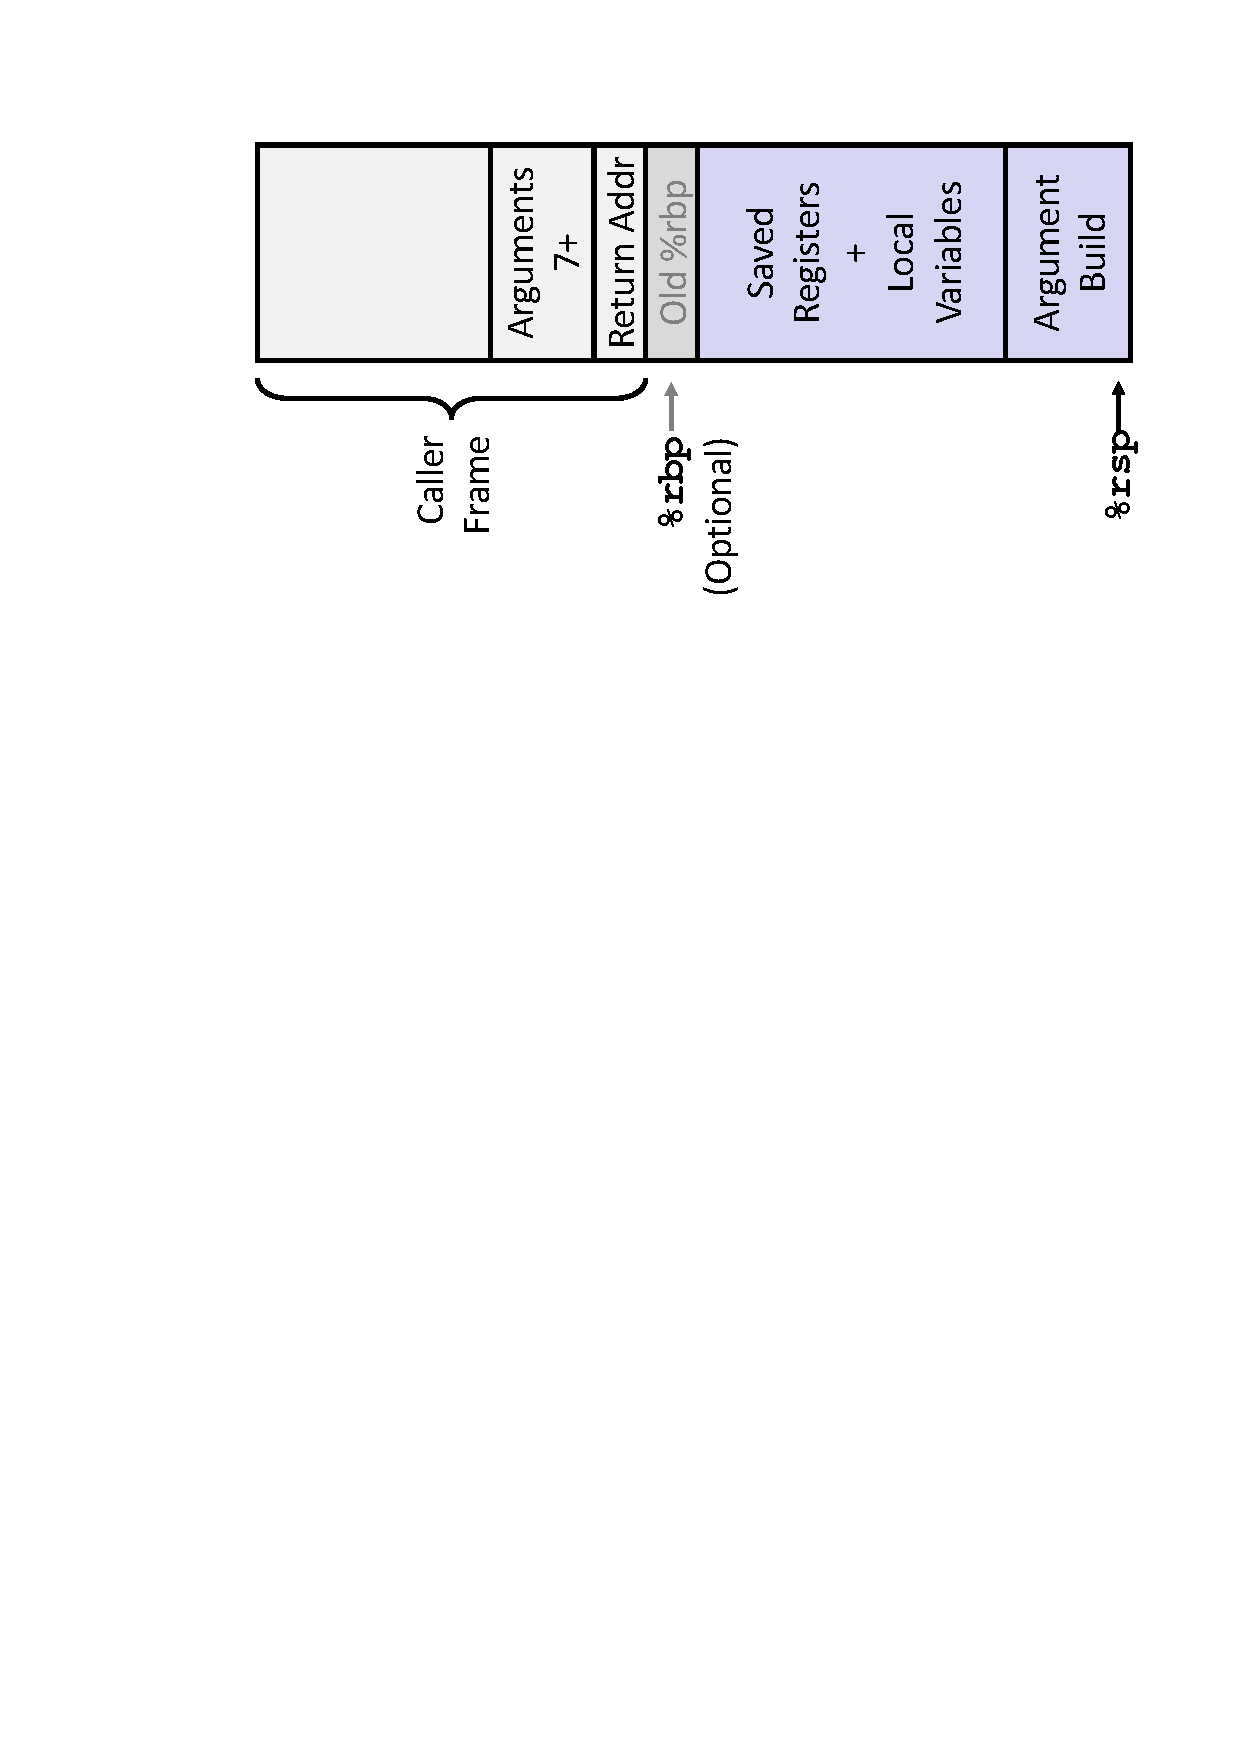
\includegraphics[width=0.8\linewidth]{machine-procedures.pdf}
\end{figure}
\end{center}
\vspace{-50pt}
\section{Machine Data}

\textbf{Data Alignment}: K-byte object at addr multiple of K
\begin{center}
    \begin{tabular}{| c || c |}
    \hline
    \textbf{Size (bytes)} & \textbf{Types}\\ \hline
    1 & \tt{char}  \\ \hline
    2 & \tt{short} \\ \hline
    4 & \tt{int, float}  \\ \hline
    8 & \tt{long, double, char *} \\ \hline
    \end{tabular} \\
\end{center}
\vspace{7pt}
\textbf{Arrays}: Element i at address \tt{\&A[0] + i * sizeof(type)}
\begin{itemize}[noitemsep, topsep=1pt]
    \item 1D array access: \tt{movl (\%rdx,\%rcx,4),\%eax} gets \tt{A[\%rcx]} for \tt{int A[]}
    \item 2D row-major: \tt{A[i][j]} at \tt{\&A + i*C*s + j*s} for \tt{A[R][C]} with size s
    \item Multi-level arrays: Array of pointers e.g., \tt{int *A[R]} for jagged arrays
\end{itemize}
\vspace{10pt}
\textbf{Structs}: Fields stored with alignment padding
\begin{itemize}[noitemsep, topsep=1pt]
    \item K-byte field must be at addr multiple of K
    \item Field alignment may require padding between fields
    \item Struct alignment = max alignment of any field
    \item Struct size = multiple of largest alignment requirement
    \item Example: \tt{struct \{char a; int b; char c;\}} $\rightarrow$ \\12 bytes
      \begin{tabular}{|c|c|c|c|c|c|c|c|c|c|c|c|} \hline
        0 & 1 & 2 & 3 & 4 & 5 & 6 & 7 & 8 & 9 & 10 & 11 \\ \hline
        a & \multicolumn{3}{c|}{pad} & \multicolumn{4}{c|}{b} & c & \multicolumn{3}{c|}{pad} \\ \hline
      \end{tabular}
    \item Nested structs: inner struct follows its own alignment rules
    \item Access field at offset d: \tt{movq d(\%rdi),\%rax}
\end{itemize}
\vspace{10pt}
\textbf{Unions}: All fields share same memory location
\begin{itemize}[noitemsep, topsep=1pt]
    \item Size = largest member size
    \item All fields have offset 0 from base address
    \item Example: \tt{union \{int i; float f; char c[4];\}} \\occupies 4 bytes total
      \begin{tabular}{|c|c|c|c|} \hline
        0 & 1 & 2 & 3 \\ \hline
        \multicolumn{4}{|c|}{i (4 bytes)} \\ \hline
        \multicolumn{4}{|c|}{f (4 bytes)} \\ \hline
        c[0] & c[1] & c[2] & c[3] \\ \hline
      \end{tabular}
    \item Access any member using base address: \tt{movl (\%rdi), \%eax}
    \item Used for type punning (e.g., \tt{u.f = 1.0f; bits = u.i}) or memory optimization
\end{itemize}